\documentclass[12pt, a4paper]{article}

\usepackage{amssymb}
\usepackage{multicol}
\usepackage{enumerate}
\usepackage[top=5em, bottom=5em, left=5em, right=5em]{geometry}
\usepackage{listings}
\usepackage{tikz}
\usetikzlibrary{positioning}

\setlength\parskip{1em}
\setlength\parindent{0em}

\title{Assignment 11}

\author{Hendrik Werner s4549775}

\begin{document}
\maketitle

\section{} %1
The minimal cut for this graph is $(\{s, A, B, C\}, \{D, t\})$ with a flow of $5$ which is also the maximum flow for the graph.

\section{} %2

An empty cell means that there is no path. You could also fill in $\infty$ everywhere.

\begin{tabular}{|c|c|c|c|c|}
	\hline
	1 & A & B & C & D\\
	\hline
	A & 0 & 7 && 2\\
	\hline
	B & 1 & 0 & 9 &\\
	\hline
	C & 4 && 0 &\\
	\hline
	D & 8 && 3 & 0\\
	\hline
\end{tabular}

\begin{tabular}{|c|c|c|c|c|}
	\hline
	2 & A & B & C & D\\
	\hline
	A & 0 & 7 && 2\\
	\hline
	B & 1 & 0 & 9 & 3\\
	\hline
	C & 4 & 11 & 0 & 6\\
	\hline
	D & 8 & 15 & 3 & 0\\
	\hline
\end{tabular}

\begin{tabular}{|c|c|c|c|c|}
	\hline
	3 & A & B & C & D\\
	\hline
	A & 0 & 7 & 16 & 2\\
	\hline
	B & 1 & 0 & 9 & 3\\
	\hline
	C & 4 & 11 & 0 & 6\\
	\hline
	D & 8 & 15 & 3 & 0\\
	\hline
\end{tabular}

\begin{tabular}{|c|c|c|c|c|}
	\hline
	4 & A & B & C & D\\
	\hline
	A & 0 & 7 & 16 & 2\\
	\hline
	B & 1 & 0 & 9 & 3\\
	\hline
	C & 4 & 11 & 0 & 6\\
	\hline
	D & 7 & 14 & 3 & 0\\
	\hline
\end{tabular}

\begin{tabular}{|c|c|c|c|c|}
	\hline
	5 & A & B & C & D\\
	\hline
	A & 0 & 7 & 5 & 2\\
	\hline
	B & 1 & 0 & 6 & 3\\
	\hline
	C & 4 & 11 & 0 & 6\\
	\hline
	D & 7 & 14 & 3 & 0\\
	\hline
\end{tabular}

\section{} %3

Graph $G$ contains two strongly connected components. The first one ($X$) consists of $A, D, E, G$ and the other one ($Y$) contains $B, C, F, H$. The component graph thus looks like this:

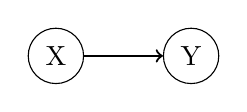
\begin{tikzpicture}[every node/.style={circle, draw, minimum width=2em}]
	\node (A) {X};
	\node [right=of A] (B) {Y};

	\draw[->, thick] (A) -- (B);
\end{tikzpicture}

\section{} %4

Initial state:

\begin{tabular}{|c|c|c|c|c|c|c|c|}
	\hline
	4 & 3 & 6 & 5 & 2 & 2 & 1 & 6\\
	\hline
\end{tabular}

Merging steps:

\begin{enumerate}
	\item \begin{tabular}{|c|c|c|c|c|c|c|c|}
		\hline
		3 & 4 & 5 & 6 & 2 & 2 & 1 & 6\\
		\hline
	\end{tabular}
	\item \begin{tabular}{|c|c|c|c|c|c|c|c|}
		\hline
		3 & 4 & 5 & 6 & 1 & 2 & 2 & 6\\
		\hline
	\end{tabular}
	\item \begin{tabular}{|c|c|c|c|c|c|c|c|}
		\hline
		1 & 2 & 2 & 3 & 4 & 5 & 6 & 6\\
		\hline
	\end{tabular}
\end{enumerate}

\section{} %5

\section{} %6

\begin{tabular}{|c|c|c|c|c|c|c|c|}
	\hline
	&& A & A & C & H & E & N\\\hline
	& 0 & 1 & 2 & 3 & 4 & 5 & 6\\\hline
	A & 1 &&&&&&\\\hline
	T & 2 &&&&&&\\\hline
	H & 3 &&&&&&\\\hline
	E & 4 &&&&&&\\\hline
	N & 5 &&&&&&\\\hline
\end{tabular}

\end{document}
